\documentclass{article}
\usepackage[pdfcreator={LaTeX}]{hyperref}
\usepackage{graphicx}
\usepackage[utf8]{inputenc} 
\usepackage[ngerman]{babel}


\usepackage{tikz}
\usetikzlibrary{arrows,shadows}
\usepackage{pgf-umlsd}


\begin{document}
\begin{titlepage}

\begin{center}
\textbf{\textsc{\LARGE Implementierungsbericht}}

{\large \today}

\vspace{2cm}
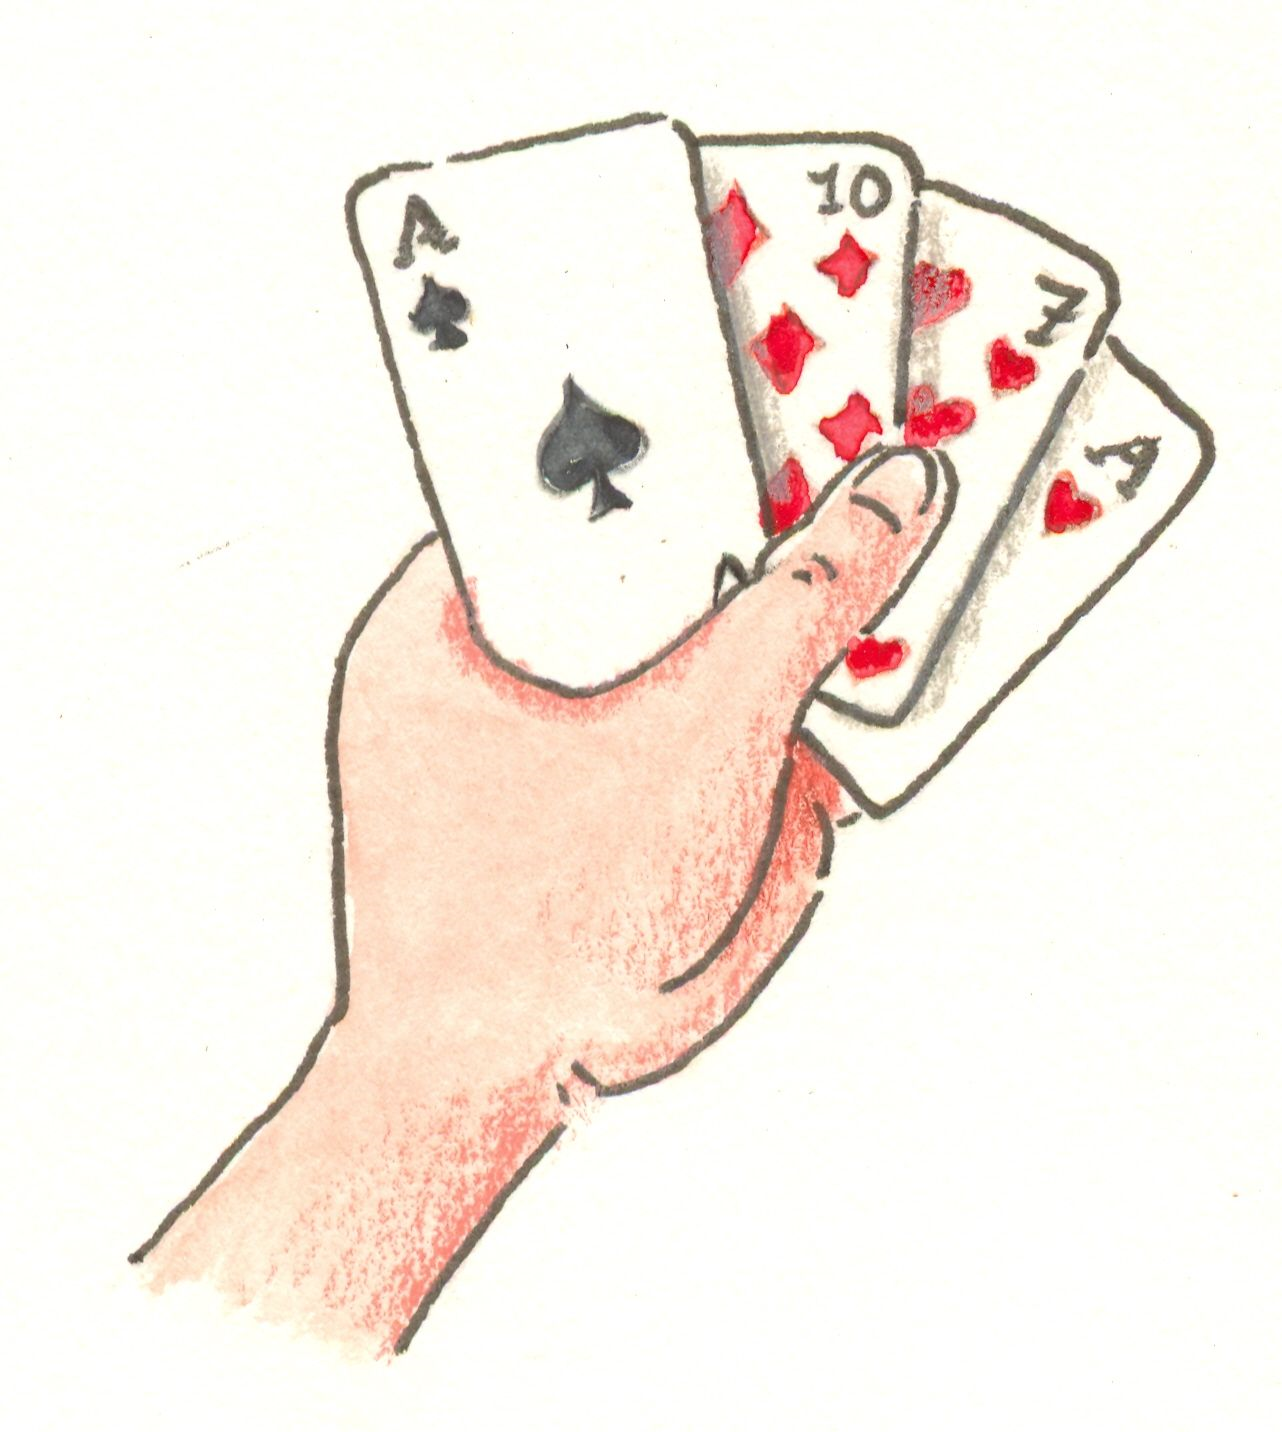
\includegraphics{kartenspiel}
\ \\
\ \\

\textbf{\textsc{\LARGE NET-WizHearts}}
\vspace{2cm}

\begin{tabular}{|c|c|c|}\hline
   Phase & Verantwortlicher & E-Mail \\ \hline\hline
   Pflichtenheft & Alina Meixl &  alina@meixl.de \\ \hline
   Entwurf & Viktoria Witka & witkaviktoria@freenet.de \\ \hline
   Spezifikation & Daniel Riedl & dariedl14@yahoo.de \\ \hline
   Implementation & Andreas Altenbuchner& a.andi007@gmail.com\\ \hline
   Verifikation & Patrick Kubin & kubin@fim.uni-passau.de\\ \hline
   Präsentation & w& w\\ \hline
 \end{tabular}

\end{center}

\end{titlepage}

\tableofcontents
\newpage

\section{Einleitung}
Dieses Dokument ist eine Dokumentation der Implementierungsphase. In Folgenden werden Änderungen aufgezählt, die seit der letzten Phase entstanden sind, des Weiteren wird eine Übersicht gegeben über die zuvor festgelegten Milestones und die tatsächliche Umsetzung dieser Aufteilung.

\section{Änderungen gegenüber der Spezifikation}

\subsection{Client}

\begin{itemize}
\item  \textbf{LanguageInterpreter:}  \textit{Neu hinzugefügte Klasse}: Wird verwendet, um Fehlermeldungen, die vom Server gesendet werden zu interpretieren und in der korrekten Sprache auszugeben.
\end{itemize}

\subsection{View}

\begin{itemize}
\item \textbf{Login:} \textit{hinzugefügt}: getUsername(), getServerAdress()
\item \textbf{Lobby:} \textit{hinzugefügt}: getChosenGameName(), getChatMessage(), hasPWChosenGame()
\item \textbf{CreateWindow:} \textit{entfernt}: addLeaveButtonListener(), addRulesetSelectionListener(); \textit{hizugefügt}: setRulesetTypes(), getGameName(), hasPassword(), getPassword(), getSelectedRulesetType()
\item \textbf{GameLobby:} \textit{hinzugefügt}: getChatMessage(), getSelectedPlayer()
\item \textbf{Game:} \textit{hinzugefügt}: getChatMessage(), addChatMessageListener() \textit{geändert}: makeTrickGameBoard()
\item \textbf{TrumpColour:} \textit{Neu hinzugefügte Klasse}: Hinzugefügt um die aktuelle Trumpfarbe anzuzeigen. Das ist primär bei Wizard wichtig, da der Zauberer selbst keine Farbe hat und dementsprechend nicht genutzt werden kann, um die Trumpffarbe anzuzeigen.
\item \textbf{Sonstiges:} Weiterhin wurden auch viele Detailänderungen an den einzelnen GamePanel Bausteinen vorgenommen.
\end{itemize}

\subsection{Ruleset}

\begin{itemize}
\item \textit{hinzugefügt} \textbf{DiscardedCard:} Eine Karte die von einem Spieler auf den Ablegestapel gelegt wird und als Atrribute die Karte die gespielt wurde und den Spieler der sie gespielt hat 
enthält.;

\item \textit{hinzugefügt} \textbf{EmptyCard:} Eine leere Karte die zu keinem Spiel gehört;

\item \textbf{GameState:} \textit{hinzugefügt}: madeTrick() Entfernt die DiscardedCards im Ablagestapel und gibt ihre Karten als Set einem Spieler in seine gemachten Stiche, restartDeck () Wird aufgerufen um ein neues Deck zu erstellen und alle Karten die vorher im Spiel waren zu löschen., nextRound() Erhöht die Rundenzahl um eins; \textit{gelöscht}: getNumberOfPlayedCards()

\item \textbf{ServerRuleset} \textit{hinzugefügt}: updatePlayers() Schickt an alle Spieler ein neues GameClientUpdate, getPlayedCards() Holt die gespielten Karten im Ablagestapel, startRound() Wird am Anfang jeder Runde aufgerufen. Mischt und verteilt Karten und schickt Comobject mit Updates und Request für den Rundenanfang., getWinners() Wird bei Spielende aufgerufen und gibt die Namen der Sieger zurück,; 

\item \textbf{ServerWizard} \textit{hinzugefügt}: trumpColour Die Trumpffarbe im Spiel; 

\item \textbf{ServerHearts:} \textit{hinzugefügt}: heartBroken: Gibt an ob Herz gebrochen wurde. swapLeft(),swapRight(),swapAcross(): Tauscht die Karten nach links, rechts oder gegenüber
\end{itemize}

\subsection{Server}
/**\\
 * LoginServer. Diese Klasse ist für das Zustandekommen von \\
 * Clientverbindungen zustaendig. Sie hat den ClientListenerTread\\
 * als innere Klasse.\\
 */\\
\begin{itemize}
\item  \textbf{LoginServer:}  \textit{Neu hinzugefügte Klasse, erbt von Server}.\\
\textit{Attribute}:  \\
/**\\
 * Ein Thread, der fuer das Annehmen neuer Clientverbindungen zustaendig ist\\
 */\\
Thread clientListenerThread\\
/**\\
 * Der LobbyServer\\
 */\\
LobbyServer lobby \\
\\
\textit{Methoden}: 
/**\\
 * Diese ueberladene Methode ueberprueft, ob der Name im Set names des\\
 * LobbyServers vorhanden ist, falls ja, wird ein ComWarning an den Client\\
 * geschickt, dass der Name bereits vergeben ist, falls nein, wird im Player\\
 * setName aufgerufen. Der Player wecheselt auf den LobbyServer, sein Name\\
 * wird in das names Set eingefügt. Dem Client wird ein ComInitLobby\\
 * geschickt.\\
 *\\
 * @param player\\
 *            ist der Thread der die Nachricht erhalten hat\\
 * @param login\\
 *            ist das ComObject, dass den Benutzernamen des Clients enthält\\
 */\\
receiveMessage(Player player, ComLoginRequest login) \\
/**\\
 * Diese Methode schliesst die Verbindung zu einem Client. Der uebergebene\\
 * Player wird aus dem playerSet sowie dem names Set im LobbyServer\\
 * entfernt.\\
 * \\
 * @param player\\
 *            ist der Spieler der entfernt wird\\
 */\\
disconnectPlayer()\\
\\
\item  \textbf{GameServer:} \textit{hinzugefügt}: \\
/**\\
 * Diese Methode beendet das Spiel und gibt die Player an den LobbyServer\\
 * zurueck.Der GameServer wird aus dem Set des LobbyServers entfernt und die\\
 * Spieler in der Lobby erhalten ein Gamelist Update.\\
 */\\
quitGame()\\
/**\\
 * Getter fuer den Namen des Spielleiters\\
 * \\
 * @return Gibt den gameMasterName zurueck\\
 */\\
getGameMasterName()\\
/**\\
 * Getter fuer das Passwort\\
 * \\
 * @return Gibt das Passwort des Spieles zurueck\\
 */\\
getPassword()\\
/**\\
 * Diese Methode verpackt eine RulesetMessage in ein ComObject und\\
 * verschickt es mit sendToPlayer() an einen bestimmten Spieler.\\
 * @param player\\
 *            ist der Name des Spielers an den die Nachricht verschickt wird\\
 * @param message\\
 *            ist die Ruleset Nachricht, die in ein ComObject verpackt wird\\
 */\\
sendRulesetMessage(String player, RulesetMessage message)\\
/**\\
 * Diese Methode verschickt ComWarning mit der übergebenen Warnung \\
 * mit broadcast() an alle Spieler.\\
 * @param message\\
 *            ist die Ruleset Nachricht, die in ein ComObject verpackt wird\\
 */\\
broadcastRulesetMessage(RulesetMessage message)\\
/**\\
 * Diese Methode verschickt ein ComWarning mit sendToPlayer() an einen bestimmten Spieler.\\
 * @param player\\
 *            ist der Name des Spielers an den die Nachricht verschickt wird\\
 * @param message\\
 *            ist die Ruleset Nachricht, die in ein ComObject verpackt wird\\
 */\\
sendWarning(String player, WarningMsg warning)\\
/**\\
 * Diese Methode verpackt eine RulesetMessage in ein ComObject und\\
 * verschickt es mit broadcast() an alle Spieler.\\
 * @param message\\
 *            ist die Ruleset Nachricht, die in ein ComObject verpackt wird\\
 */\\
broadcastWarning(WarningMsg warning) \\
/**\\
 * Gibt zurück, ob das Spiel bereits gestartet ist\\
 * @return den Wert von hasStarted\\
 */\\
isHasStarted()\\
/**\\
 * Setter für has started\\
 * @param hasStarted wird auf den übergebenen Wert gesetzt\\
 */\\
setHasStarted(boolean hasStarted)\\
\textit{entfernt}: \\
receiveMessage(Player player, ComClientQuit quit)--wird jetzt mit receiveMessage(Player player, ComClientLeave leave) gelöst
\\
\item  \textbf{GameServerRepresentation:} \textit{implementiert jetzt Serializable}\\
\\
\item  \textbf{LobbyServer:} \textit{entfernt}: 
innere Klasse ClientListenerThread--- ist jetzt im Login Server\\
Set<Player> noNames--- wurde nicht gebraucht bzw. wurde durch den LoginServer einfacher gelöst\\
 ServerSocket socket--- ist jetzt im Login Server\\
receiveMessage(Player player, ComClientQuit quit )--- macht der allgemeine Server\\
receiveMessage(Player player, ComLoginRequest login)--- ist jetzt im Login Server\\
\textit{hinzugefügt}:\\
/**\\
 * Hilfsmethode, die einen Spieler zu einem Spiel hinzufuegt\\
 * \\
 * @param player ist der Spieler, der hinzugefügt wird\\
 * @param game ist das Spiel zu dem der Spieler hinzugefügt wird\\
 */\\
 addPlayerToGame(Player player, GameServer game)\\
/**\\
 * Getter für das Set der Spielernamen\\
 * \\
 * @return Gibt das names Set zurück\\
 */\\
getNames()\\
\\
\item  \textbf{ClientListenerThread:} erbt jetzt von Thread  \textit{hinzugefügt}:\\
/**\\
 * Zeigt, ob der Tread auf verbindungen wartet\\
 */\\
boolean waiting\\
ServerSocket socket\\
LoginServer server\\
\\
\item  \textbf{Player:}  erbt jetzt von Thread  \textit{hinzugefügt}: \\
/**\\
 * Socket des Clients\\
 */\\
Socket connection\\
/**\\
 * Zeigt an, ob der Thread läuft\\
 */\\
boolean run\\
/**\\
 * Diese Methode schließt den Socket, sowie comIn und comOut\\
 */\\
closeConnection()\\

\textit{geändert}: getName() heißt getPlayerName(), setName() heißt setPlayerName()
\\
\item  \textbf{Server:} \textit{hinzugefügt}: eine receiveMessage Methode für jedes ComObject, das vom Server empfangen werden soll; \\
\textit{geändert}: handleIOException heißt jetzt disconnectPlayer()
\\
\item  \textbf{ServerMain:} \textit{hinzugefügt}:\\
 Attribut LoginServer loginServer\\
\end{itemize}

\subsection{ComObjects}

\begin{itemize}
\item 
\end{itemize}

\newpage

\section{Vergleich: Implementierungsplan und Realität}

\subsection{Änderungen am Plan}
\begin{itemize}
\item Zuständigkeit von Arbeitspaket Client(Lobby) wurde von Patrick an Andi gegeben, um die Arbeitszeiten anzugleichen
\item Zuständigkeit von Arbeitspaket Ruleset(Wizard-Client) wurde von Patrick/Andi and Daniel gegeben, um die Arbeitszzeiten anzugleichen
\end{itemize}

\subsection{Milestone 1}

\begin{tabular}{|c|c|c|c|c|}\hline
   Bereich & angen. Dauer & tats. Dauer & Abweichung & Begründung \\ \hline\hline
   View(Login+Lobby) & 8 Stunden & 4 Stunden & 50\% & (1) \\ \hline
   View(Create+Join) & 8 Stunden & 5 Stunden & 37,5\% & (1)\\ \hline
   View(GameLobby) & 8 Stunden & 3 Stunden & 62,6\% & (1)\\ \hline
   Client(Login) & 8 Stunden & 8,5 Stunden & (-) 6,25\% & (2) \\ \hline
   Client(Lobby) & 8 Stunden &  6,5 Stunden & 18,75\% &\\ \hline
   Client(Create+Join) &  8 Stunden & 6 Stunden & 25\% &\\ \hline
   Server(Login) & 16 Stunden & 6 Stunden & 62,5\% & (5) \\ \hline
   Server(Lobby) & 8 Stunden & 3 Stunden & 62,5\% & (5)\\ \hline 
   Server(Create+Join) & 12 Stunden & 6 Stunden & 50\% & (5)\\ \hline 
   Ruleset(Daten) & 20 Stunden & 6 Stunden & 25\% & (4) \\ \hline 
   Ruleset(ServerWizard) & 30 Stunden & 24 Stunden & 33,4\% &\\ \hline 
 \end{tabular}

\begin{itemize}
\item \textbf{(1)} Es waren noch Code-Teile aus der Pflichtenheft-Phase vorhanden. \\
\item \textbf{(2)} Login wegen Änderungen am Loginserver umgebaut. \\
\item \textbf{(3)} Viele der ComObjects waren bereits fertig. \\
\item \textbf{(4)} Wurde hauptsächlich schon in Spezifikationsphase implementiert. \\
\item \textbf{(5)} Stundenzahl würde Anfangs verdoppelt. \\
\end{itemize}

\subsection{Milestone 2}

\begin{tabular}{|c|c|c|c|c|}\hline
   Bereich & angen. Dauer & tats. Dauer & Abweichung & Begründung\\ \hline\hline
   View(Game) & 20 Stunden & 18,5 Stunden & 7,5\% &\\ \hline 
   Client (GameLobby) &  8 Stunden & 10 Stunden & (-) 25\% &\\ \hline
   Server(GameLobby) & 10 Stunden & 5 Stunden & 50\% &(5)\\ \hline
   Ruleset(ServerHearts) & 30 Stunden & 18 Stunden & 50\% &\\ \hline 
   Handbuch & - & 5 Stunden & - &\\ \hline 
 \end{tabular}

\subsection{Milestone 3}

\begin{tabular}{|c|c|c|c|c|}\hline
   Bereich & angen. Dauer & tats. Dauer & Abweichung & Begründung\\ \hline\hline
   View(WizardWindows) & 4 Stunden & 3,5 Stunden & 12,5\% &\\ \hline
   View(HeartsWindows) & 4 Stunden & 3 Stunden & 25\% &\\ \hline
   Client (Game) & 14  Stunden &  12 Stunden & 14,3\% & (1)\\ \hline
   Ruleset(ClientWizard) & 6 Stunden & 5 Stunden & 16,7\% &\\ \hline 
   Ruleset(ClientHearts) & 6 Stunden & 5 Stunden & 16,7\% &\\ \hline 
   Server(Game) & 4 Stunden & 2,5 Stunden & 37,5\% &\\ \hline
   Client(LanguageInterpreter) & - & 2 Stunden & - &\\ \hline
   Karten & - & 4 Stunden & - &\\ \hline
   Handbuch & - & 2 Stunden & - &\\ \hline
 \end{tabular}

\begin{itemize}
\item \textbf{(1)} Regelwerk Packete delegiert. Zeit für Refactoring des Clientcodes verwendet. \\
\end{itemize}

\subsection{Finale Phase}
\begin{tabular}{|c|c|c|c|c|}\hline
   Bereich & angen. Dauer & tats. Dauer & Abweichung & Begründung\\ \hline\hline
   View(Polishing) & 10 Stunden & 7,5 Stunden & 25\% &\\ \hline
   Client(Polishing) & 10 Stunden & 12 Stunden & 20\% & (1) \\ \hline
   Ruleset(Polishing & 10 STunden & 5 Stunden & 50\% &\\ \hline
   Server(Polishing) & 10 Stunden & 1 Stunde & 25\% &\\ \hline
 Handbuch & - & 2 Stunden & - &\\ \hline
 
 \end{tabular}
 
 \begin{itemize}
\item \textbf{(1)} Nacharbeiten wegen Nebenläufigkeit und JUnit Tests sowie Tests in Gruppe wegen Abgabe\\
\end{itemize}
 
 \section{Bekannte Bugs}


\end{document}
